% Auto-generated by writeup/figs/economy_ising/generate.py.
\providecommand{\cvunit}{1.05cm}
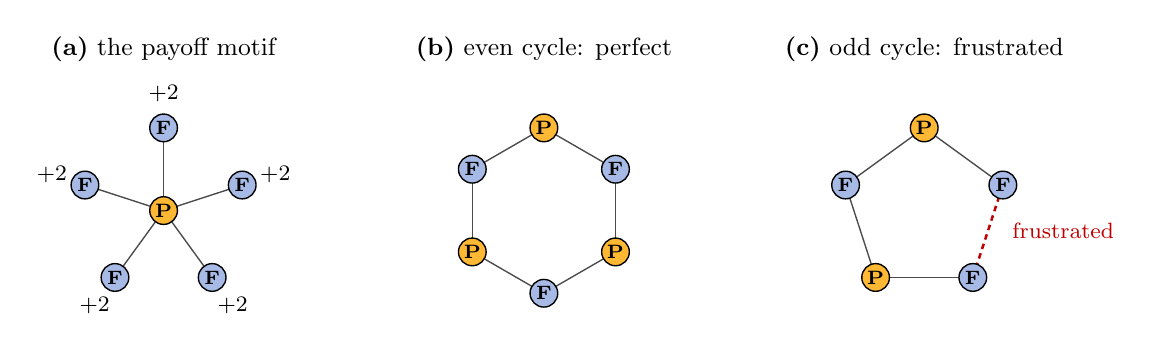
\begin{tikzpicture}[
    x=\cvunit, y=\cvunit,
    panelframe/.style={draw=black!85, line width=0.5pt},
    paneltitle/.style={font=\small},
    factory/.style={fill=cyan!45!blue!35, draw=black, line width=0.5pt},
    pplant/.style={fill=orange!70!yellow!80, draw=black, line width=0.5pt},
    ours/.style={fill=cyan!45!blue!35, draw=black, line width=0.5pt},
    enemy/.style={fill=red!45, draw=black, line width=0.5pt},
    neutral/.style={fill=black!12, draw=black, line width=0.5pt},
    gedge/.style={draw=black!70, line width=0.5pt},
    frustrated/.style={draw=red!75!black, line width=0.9pt, dash pattern=on 2pt off 1.6pt},
    frontline/.style={draw=black!55, line width=0.7pt, dash pattern=on 3.5pt off 2.5pt},
    flow/.style={-{Stealth[length=4.5pt]}, draw=black!75, line width=0.7pt},
    consign/.style={-{Stealth[length=5pt]}, draw=green!55!black, line width=0.8pt},
    chosen/.style={draw=green!55!black, line width=1.0pt},
    note/.style={font=\small},
    smallnote/.style={font=\footnotesize},
  ]
  \begin{scope}[shift={(0,0)}]
    \draw[gedge] (0.0000,0.0000) -- (0.0000,1.0000);
    \draw[gedge] (0.0000,0.0000) -- (-0.9511,0.3090);
    \draw[gedge] (0.0000,0.0000) -- (-0.5878,-0.8090);
    \draw[gedge] (0.0000,0.0000) -- (0.5878,-0.8090);
    \draw[gedge] (0.0000,0.0000) -- (0.9511,0.3090);
    \filldraw[factory] (0.0000,1.0000) circle (5pt);
    \node[anchor=center] at (0.0000,1.0000) {\scriptsize\textbf{F}};
    \node[anchor=center] at (0.0000,1.4200) {\footnotesize$+2$};
    \filldraw[factory] (-0.9511,0.3090) circle (5pt);
    \node[anchor=center] at (-0.9511,0.3090) {\scriptsize\textbf{F}};
    \node[anchor=center] at (-1.3505,0.4388) {\footnotesize$+2$};
    \filldraw[factory] (-0.5878,-0.8090) circle (5pt);
    \node[anchor=center] at (-0.5878,-0.8090) {\scriptsize\textbf{F}};
    \node[anchor=center] at (-0.8347,-1.1488) {\footnotesize$+2$};
    \filldraw[factory] (0.5878,-0.8090) circle (5pt);
    \node[anchor=center] at (0.5878,-0.8090) {\scriptsize\textbf{F}};
    \node[anchor=center] at (0.8347,-1.1488) {\footnotesize$+2$};
    \filldraw[factory] (0.9511,0.3090) circle (5pt);
    \node[anchor=center] at (0.9511,0.3090) {\scriptsize\textbf{F}};
    \node[anchor=center] at (1.3505,0.4388) {\footnotesize$+2$};
    \filldraw[pplant] (0.0000,0.0000) circle (5pt);
    \node[anchor=center] at (0.0000,0.0000) {\scriptsize\textbf{P}};
    \node[anchor=center] at (0.0000,1.9500) {\small\textbf{(a)} the payoff motif};
  \end{scope}
  \begin{scope}[shift={(4.6,0)}]
    \draw[gedge] (0.0000,1.0000) -- (-0.8660,0.5000);
    \draw[gedge] (-0.8660,0.5000) -- (-0.8660,-0.5000);
    \draw[gedge] (-0.8660,-0.5000) -- (-0.0000,-1.0000);
    \draw[gedge] (-0.0000,-1.0000) -- (0.8660,-0.5000);
    \draw[gedge] (0.8660,-0.5000) -- (0.8660,0.5000);
    \draw[gedge] (0.8660,0.5000) -- (0.0000,1.0000);
    \filldraw[pplant] (0.0000,1.0000) circle (5pt);
    \node[anchor=center] at (0.0000,1.0000) {\scriptsize\textbf{P}};
    \filldraw[factory] (-0.8660,0.5000) circle (5pt);
    \node[anchor=center] at (-0.8660,0.5000) {\scriptsize\textbf{F}};
    \filldraw[pplant] (-0.8660,-0.5000) circle (5pt);
    \node[anchor=center] at (-0.8660,-0.5000) {\scriptsize\textbf{P}};
    \filldraw[factory] (-0.0000,-1.0000) circle (5pt);
    \node[anchor=center] at (-0.0000,-1.0000) {\scriptsize\textbf{F}};
    \filldraw[pplant] (0.8660,-0.5000) circle (5pt);
    \node[anchor=center] at (0.8660,-0.5000) {\scriptsize\textbf{P}};
    \filldraw[factory] (0.8660,0.5000) circle (5pt);
    \node[anchor=center] at (0.8660,0.5000) {\scriptsize\textbf{F}};
    \node[anchor=center] at (0.0000,1.9500) {\small\textbf{(b)} even cycle: perfect};
  \end{scope}
  \begin{scope}[shift={(9.2,0)}]
    \draw[gedge] (0.0000,1.0000) -- (-0.9511,0.3090);
    \draw[gedge] (-0.9511,0.3090) -- (-0.5878,-0.8090);
    \draw[gedge] (-0.5878,-0.8090) -- (0.5878,-0.8090);
    \draw[frustrated] (0.5878,-0.8090) -- (0.9511,0.3090);
    \draw[gedge] (0.9511,0.3090) -- (0.0000,1.0000);
    \filldraw[pplant] (0.0000,1.0000) circle (5pt);
    \node[anchor=center] at (0.0000,1.0000) {\scriptsize\textbf{P}};
    \filldraw[factory] (-0.9511,0.3090) circle (5pt);
    \node[anchor=center] at (-0.9511,0.3090) {\scriptsize\textbf{F}};
    \filldraw[pplant] (-0.5878,-0.8090) circle (5pt);
    \node[anchor=center] at (-0.5878,-0.8090) {\scriptsize\textbf{P}};
    \filldraw[factory] (0.5878,-0.8090) circle (5pt);
    \node[anchor=center] at (0.5878,-0.8090) {\scriptsize\textbf{F}};
    \filldraw[factory] (0.9511,0.3090) circle (5pt);
    \node[anchor=center] at (0.9511,0.3090) {\scriptsize\textbf{F}};
    \node[anchor=west] at (0.9494,-0.2500) {\footnotesize\textcolor{red!75!black}{frustrated}};
    \node[anchor=center] at (0.0000,1.9500) {\small\textbf{(c)} odd cycle: frustrated};
  \end{scope}
\end{tikzpicture}%
